\subsection{Scriptable Entity}
\label{sub:Scriptable Entity}

\subsubsection{前言}
RishEngine 支援開發者使用引擎提供之 API 撰寫遊戲邏輯,並使用編輯器將寫好的邏輯綁定在多個遊戲物件上,構成可以互動的遊戲場景(Scene)。

\subsubsection{實作}
\begin{figure}[h]
    \begin{center}
    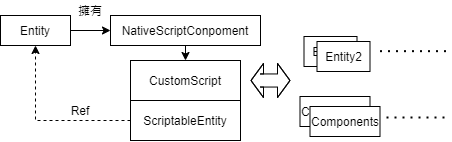
\includegraphics[width=0.6\textwidth]{./resources/scriptable/implement.png}
    \end{center}
\caption{展示圖}
\label{fig:implement}
\end{figure}

原本引擎在 ECS 中的 Entity 是代表遊戲物件,而 ScriptableEntity 代表被 Script 所操控的 Entity。

\begin{lstlisting}
class ScriptableEntity
{
public:
    ScriptableEntity() = default;
    virtual ~ScriptableEntity() = default;

    // Main Functions
    virtual void onCreate() {}
    virtual void onDestroy() {}
    virtual void onUpdate(Time dt) = 0;
    virtual void onImGuiRender() = 0;

    // Virtual Constructor Pattern
    template<class Derived>
    Derived* clone() const
    {
        return new Derived(// new type Derived
            static_cast<const Derived &>(*this) // cast to derived type
        );
    }
private:
    Entity m_entity;
};
\end{lstlisting}

如果要實作一個 Script 時,要繼承 ScriptableEntity 並實作其提供的介面,onCreate() 會在 Script 建立時被執行、onUpdate() 每 frame 會執行一次、onImGuiRender() 則是用於 Editor 時可以調參數、onDestroy() 則是在 Script 被銷毀前會執行。

\begin{lstlisting}
class ExampleScript : public ScriptableEntity
{
public:
    virtual void onCreate() override
    {
    }
    virtual void onDestroy() override
    {
    }
    virtual void onUpdate(Time dt) override
    {
    	/* Update the Entity */
    }
    virtual void onImGuiRender() override
    {
    	/* Update UI in Editor */
    }
};
\end{lstlisting}

但因為我們現在引擎是採用 ECS 架構,所以還要有一個 Component 讓 Entity 擁有。定義 NativeScriptComponent 有三個資料\: instance 是 ScriptableEntity 也就是實際邏輯的 Object、scriptName 是 Script 的名稱,預設是 rl\:\:EmptyScript、valid 則代表該 Script 是否初始化。

% \footnote{entt\:\:type\_info\<T\>\:\:name\(\) 是我們使用的一個 ECS 函式庫提供的 RTTI 的函式,可以拿到一個 Type 的名稱}

% 提供了兩個函式\:bind\(\) 和 unbind\(\) 分別是綁定和解除綁定。在 bind\(\) 時會初始化參數和指定正確的 entity,因為 Script 內可能會去拿當前 Entity 的其他 Component \(例如位置、旋轉、速度等\),所以必須在初始化時綁定好;而 unbind\(\) 就是刪除 ScriptableEntity 。

\begin{lstlisting}
struct NativeScriptComponent
{
    ScriptableEntity* instance = nullptr;
    std::string scriptName     = std::string{entt::type_info<EmptyScript>::name()};
    bool valid                 = false;

    NativeScriptComponent() = default;
    ~NativeScriptComponent() = default;

    template<typename T, typename ... Args>
    void bind(Entity entity, Args&& ... args)
    {
        if(instance)
        {
            delete instance;
            instance = nullptr;
        }
        //
        scriptName = entt::type_info<T>::name();
        instance = new T(std::forward<Args>(args)...);
        instance->m_entity = entity;
    }

    void unbind()
    {
        delete instance;
        instance = nullptr;
    }
};
\end{lstlisting}

將一個 Entity 加上 NativeScriptComponent 在引擎 API 使用起來像這樣:

\begin{lstlisting}
// 新增一個叫 Player 的 Entity
Entity ent = scene->createEntity("player");
// 加入 NativeScriptComponent 並綁定 ExampleScript
ent.addComponent<NativeScriptComponent>().bind<ExampleScript>();
\end{lstlisting}

\begin{figure}[h]
    \begin{center}
    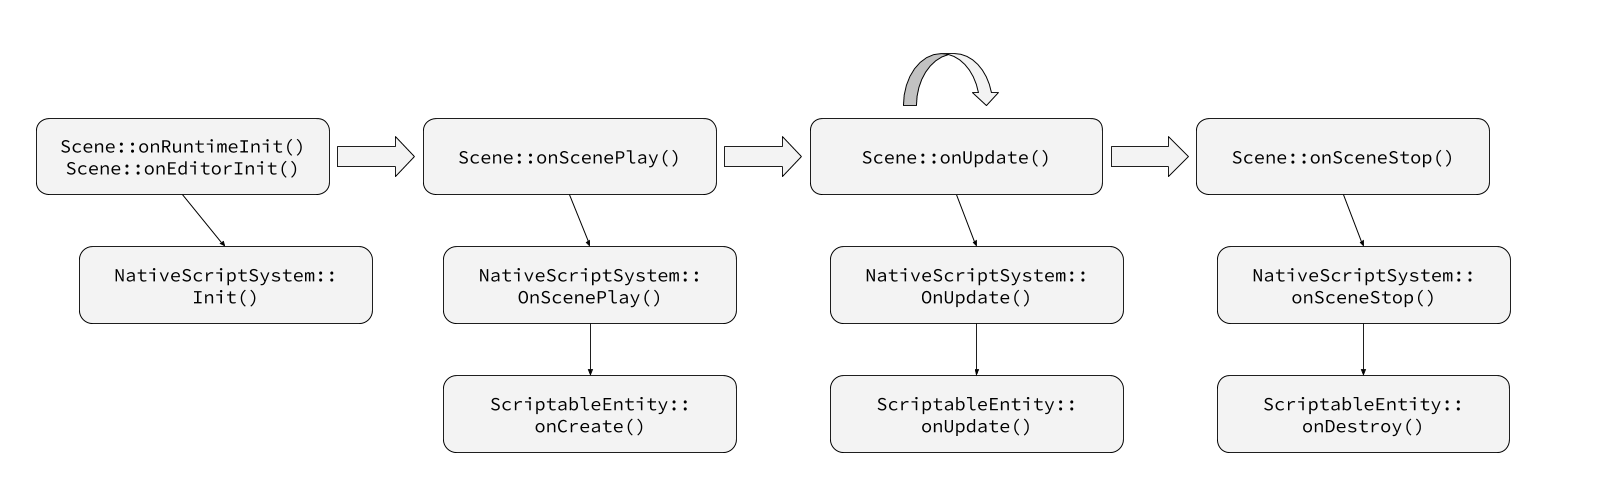
\includegraphics[width=0.6\textwidth]{./resources/scriptable/process.png}
    \end{center}
\caption{流程圖}
\label{fig:process}
\end{figure}

在引擎的流程中,在 onScenePlay\(\) 時,會初始化 Scene ,以及所有 System 其中就包含了 NativeScriptSystem 其中會呼叫 NativeScript 的 OnCreate() 初始化該 Script ,接著每次 loop 會呼叫 OnUpdate() 執行 Script 的邏輯。在要 Script 要結束時(主動結束或是被動結束)會呼叫 OnDestroy() 來清理該 Script。

在 RishEditor 中,可以使用 UI 替一個遊戲物件\(Entity\)加上 NativeScriptComponent

\subsubsection{Workflow}

如何在 RishEngine 上新增自己的 Script 呢? 首先要先撰寫一個繼承自 ScriptableEntity 的 class 例如撰寫角色的移動邏輯

\begin{lstlisting}
class PlayerController : public ScriptableEntity
{
public:
    void onUpdate(Time dt) override
    {
        auto &transform = GetComponent<TransformComponent>();
        /* Player movement code */
        if(Input::IsKeyPressed(Keyboard::Left))
            transform.translate.x -= dt * 10.f;
        /* ... */
    }
}
\end{lstlisting}

\subsubsection{未來展望}

\begin{itemize}
\item{使用 Scripting Language}
    \SubItem{目前 RishEngine 直接使用 C++ 作為 Script 的語言,優點是可以直接使用引擎的 C++ API,但缺點就是編譯非常花時間}
    \SubItem{可以使用開源的專案,接著只要提供該語言的引擎 API 之後,便可以用該腳本語言撰寫遊戲邏輯}
        % \SubSubItem{例如 mono\(C#\)\、sol2\(lua\)\、pybind11\(python\) 綁定腳本語言}
    \SubItem{動態語言雖然效能沒有編譯語言好,但動態語言不用等待編譯,這對需要快速迭代的遊戲來說至關重要}
\end{itemize}


\newpage
